\documentclass[draft]{agujournal2018}
\journalname{JGR: Earth Surface}

\usepackage{apacite}
\usepackage{amsmath,amssymb,amsfonts,amsthm}
\usepackage{comment}
\usepackage{wrapfig}
\usepackage{lipsum}
\usepackage{booktabs} % for wrapping text around tabulars in 
\usepackage{ragged2e}
\usepackage{lineno}
\usepackage[utf8]{inputenc}

% reduce white space after tables
%\usepackage[belowskip=-15pt,aboveskip=0pt]{caption}
\setlength{\intextsep}{10pt plus 2pt minus 2pt}
\setlength{\textfloatsep}{30pt}

\raggedbottom 

\justifying
\linenumbers


% there is a bug with align environments in conjunction with lineno
% the patch is 
\newcommand*\patchAmsMathEnvironmentForLineno[1]{%
	\expandafter\let\csname old#1\expandafter\endcsname\csname #1\endcsname
	\expandafter\let\csname oldend#1\expandafter\endcsname\csname end#1\endcsname
	\renewenvironment{#1}%
	{\linenomath\csname old#1\endcsname}%
	{\csname oldend#1\endcsname\endlinenomath}}% 
\newcommand*\patchBothAmsMathEnvironmentsForLineno[1]{%
	\patchAmsMathEnvironmentForLineno{#1}%
	\patchAmsMathEnvironmentForLineno{#1*}}%
\AtBeginDocument{%
	\patchBothAmsMathEnvironmentsForLineno{equation}%
	\patchBothAmsMathEnvironmentsForLineno{align}%
	\patchBothAmsMathEnvironmentsForLineno{flalign}%
	\patchBothAmsMathEnvironmentsForLineno{alignat}%
	\patchBothAmsMathEnvironmentsForLineno{gather}%
	\patchBothAmsMathEnvironmentsForLineno{multline}%
}
% from https://tex.stackexchange.com/questions/43648/why-doesnt-lineno-number-a-paragraph-when-it-is-followed-by-an-align-equation?noredirect=1&lq=1


\begin{document}

\title{Joint stochastic bedload transport and bed elevation model: variance regulation and power-law rests}
\authors{J. Kevin Pierce\affil{1}\thanks{Vancouver, British Columbia, Canada}, and Marwan A. Hassan\affil{1}}
\affiliation{1}{Department of Geography, University of British Columbia}
\correspondingauthor{James K. Pierce}{kpierce@alumni.ubc.ca}

\begin{keypoints}
\item Two species stochastic population model describes fluvial bedload particle activity and local bed elevations
\item Model predicts elevation dependent transport statistics and power-law distributed resting times for sediment undergoing burial
\item Results imply elevation changes shift particle activity fluctuations by up to 90\% and sediment rests can generate anomalous bedload diffusion
\end{keypoints}

\begin{abstract}
We describe the joint dynamics of bedload transport and bed elevation changes with a stochastic population model, and we analyze (1) the dependence of bedload flux statistics on local bed elevations and (2) resting time distributions for sediment undergoing burial in the fluctuating sedimentary bed.
The model exhibits suppression of the statistical moments of the bedload flux the bed is in a locally aggraded state and enhancement of the moments when the bed is in a degraded state.
This variance regulation effect is contingent on collective entrainment, whereby moving grains destabilize stationary grains in a positive feedback. 
When collective entrainment is turned off, the variance regulation disappears.
Return times from above in the bed elevation time-series provide heavy tailed power-law distributions of resting times with tail behavior characterized by the mean erosion rate and the active layer depth.
These results imply bedload statistics measurements on relatively short timescales can be strongly biased by bed elevation changes, and they support the growing consensus that sediment burial generates heavy tailed sediment resting times that ultimately generate anomalous bedload diffusion.
\end{abstract} 

\section{Introduction}
The transport characteristics of coarse grains moving under a turbulent flow ultimately control a wide set processes within rivers, including the export of contaminants \citep{Malmon2005,Macklin2006}, the success of ecological restoration efforts \citep{Gaeuman2017}, and the response of channel morphology to disturbances \citep{Hassan2017}.
Although the displacements of individual grains are certainly a mechanical consequence of forces imparted from the flow, bed, and other grains \citep{Wiberg1985, Vowinckel2014,Gonzalez2017}, accurately characterizing these forces within natural channels is practically impossible, especially considering the intense variability these forces display \citep{Schmeeckle2007,Celik2010, Dwivedi2011}. In response, investigators have developed a stochastic concept of bedload transport \citep{Einstein1937}, whereby the erosion and deposition of individual grains are modeled as the random results of undetermined forces \citep{Einstein1950,Paintal1971,Ancey2006}.

Essentially two types of bedload transport model have been developed from this concept. 
The first type provides the probabilistic dynamics of a small population of tracer grains as they transport downstream \citep{Einstein1937,Hubbell1964, Nakagawa1976,Martin2012,Lajeunesse2018,Wu2019}, while the second provides the statistics of the number of moving grains (``the particle activity'') within a control volume \citep{Einstein1950,Ancey2006,Ancey2008,Furbish2012a}.
In the first type, individual displacements are considered to result from alternate step-rest sequences, where step lengths and resting times are random variables following statistical distributions \citep{Einstein1937}. 
Differences between the random-walk motions of one grain and the next imply a spreading apart of tracer grains as they transport downstream: bedload tracers undergo diffusion.

Resting time distributions have been carefully studied in relation to these models because the predicted diffusion characteristics are critically dependent on whether the distribution has a light or heavy tail \citep{Bradley2017,Martin2012,Weeks1998}.
Resting times have puzzled researchers because early experiments show exponential distributions \citep{Einstein1937,Hubbell1964, Yano1969,Nakagawa1976}, while later experiments show heavy-tailed power-law distributions \citep{Martin2012,Voepel2013, Olinde2015, Pretzlav2016, Bradley2017, Liu2019}.
A predominant hypothesis is that power-law distributed resting times originate from buried grains \citep{Martin2014,Voepel2013}; this hypothesis permits surface grains to retain exponential resting times. 
Conceptually, when grains rest on the surface, material transported from upstream can deposit on top of them, preventing entrainment until its removal, driving up resting times and imparting a heavy tail to the distribution.
To our knowledge, \citet{Martin2014} have provided the only direct support for this hypothesis by tracking grains through complete cycles of burial and exhumation using a narrow flume with glass walls.
They observed heavy-tailed resting times of buried grains and described their results with a mathematical model similar to an earlier effort by \citet{Voepel2013}.
Both of these models treat bed elevation changes as a random walk and interpret resting times as return periods from above in the bed elevation time-series \citep{Redner2007}. Each describes resting time distributions from different experiments, but they rely on different random walk models, and their treatment of bed elevations as a process independent of sediment transport is questionable at first glance, since bedload transport is the source of bed elevation changes \citep{Wong2007}, and neither model explicitly includes bedload transport.
Models of sedimentary bed evolution incorporating sediment transport processes might enhance understanding of sediment resting times. 

The second type of stochastic model prescribes rates (probabilities per unit time) to the erosion and deposition events of individual grains within a control volume to calculate the particle activity \citep{Einstein1950}.
These approaches aim at a complete statistical characterization of the bedload flux \citep{Furbish2012a,Fathel2015,Furbish2017,Heyman2016}, including probability distributions \citep{Ancey2006,Ancey2008}, spatial and temporal characteristics of its fluctuations \citep{Ancey2008, Heyman2014a, Roseberry2012,Dhont2018}, and the dependence of these statistical characteristics on the length and time scales over which they are measured or calculated \citep{Singh2009,Singh2012,Saletti2015a,Ma2014}.
A recent surge in research activity has generated rapid progress and spawned many new inquiries in this subject. 
For example, \citet{Ancey2006} demonstrated that a constant erosion rate as originally proposed by \citet{Einstein1950} was insufficient to develop realistically large particle activity fluctuations, so they added a positive feedback between the particle activity and erosion rate they called ``collective entrainment'' \citep{Ancey2008, Heyman2013,Heyman2014,Ma2014, Lee2018}.
While they deemed this feedback necessary to model realistic activity fluctuations, the implications of this collective entrainment term on bed topography and particle activity changes has not been fully explored.

In this work, we present the first stochastic model coupling the erosion and deposition of individual bedload grains to local bed elevation changes.
Our model extends the \citet{Ancey2008} model to describe the interplay between bedload flux and bed elevation fluctuations in a control volume.
This development permits a systematic study of the repercussions of collective entrainment, and it frames bed elevation changes as a direct consequence of the sediment transport process.
Our model has two key assumptions: (1) bedload erosion and deposition can be characterized by probabilities per unit time, or rates \citep{Einstein1950, Ancey2008}; and (2) these rates are contingent on the local bed elevation, encoding the property that erosion of sediment is emphasized from regions of exposure, while deposition is emphasized in regions of shelter \citep{Sawai1987, Wong2007}.
We study statistical characteristics of bedload transport, bed elevation, and resting times of sediment undergoing burial using a mixture of numerical simulations and analytical approximations. We introduce the stochastic model in section \ref{sec:model}, and we solve it in section \ref{sec:solution} with a mixture of numerical and analytical techniques. We discern several new features of particle activity and bed elevation statistics that result from feedbacks between the erosion and deposition rates and the local bed elevation. We present these features in section \ref{sec:results}. We conclude with the implications of our results and speculate on topics for future research in sections \ref{sec:discussion} and \ref{sec:conclusion}.


\section{Stochastic model of bedload transport and bed elevations}
\label{sec:model}

We prescribe a volume of downstream length $L$ containing some number $n$ of moving particles in the flow and some number $m$ of stationary particles composing the bed at time $t$, as depicted in figure \ref{fig:definition}. We define $m$ relative to the mean number of grains within the control volume, so that it can be either positive or negative. $n$ is always a positive integer including $0$.
For simplicity, we consider all particles as approximately spherical with the same diameter $2a$, so their mobility and packing characteristics are consistent.
Following \citet{Ancey2008}, we prescribe four events that can occur at any instant to modify the populations $n$ and $m$, and we characterize these events using probabilities per unit time (rates).
These events are (1) migration of a moving particle into the volume from upstream ($n \rightarrow n+1$), (2) the entrainment (erosion) of a stationary particle into motion within the volume ($m\rightarrow m-1$ and $n\rightarrow n+1$), (3) the deposition of a moving particle to rest within the volume ($m\rightarrow m+1$ and $n\rightarrow n-1$), and (4) the migration of a moving particle out of the volume to downstream ($n\rightarrow n-1$).
The four events are depicted as arrows in figure \ref{fig:definition}.
As the events occur at random intervals, they set up a joint stochastic evolution of the populations $n$ and $m$ characterized by a joint probability distribution $P(n,m,t)$ for the number of particles in motion and rest in the volume at $t$.
\begin{figure}[!ht]
	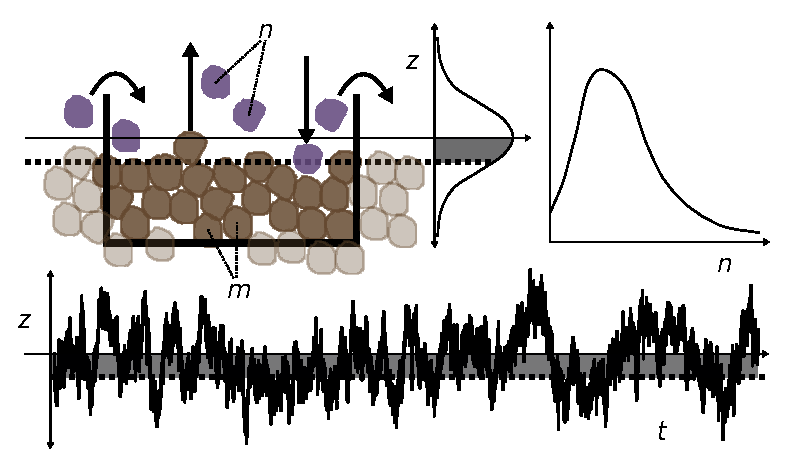
\includegraphics[width=\linewidth,keepaspectratio]{definition.pdf}
	\caption{Definition sketch of a control volume containing $n$ moving grains and $m$ resting grains. Migration, entrainment, and deposition are represented by arrows, and the instantaneous bed elevation is depicted by dotted lines. The bed is displayed in a degraded state, where $m<0$. The marginal distributions of $n$ and $m$ are indicated in the upper right panel, while the bottom panel is a realized time-series of bed elevations computed from $m$ using (\ref{eq:ele}).}
	\label{fig:definition}
\end{figure}
The populations $n$ and $m$ provide the bulk bedload flux $q_s$ and the local bed elevation $z$.
The mean bedload transport rate is given by $q_s = u_s\langle n \rangle/L$, where $u_s$ is the characteristic velocity of moving bedload and $\langle n \rangle = 
\sum_{n,m}nP(n,m) $ is the mean number of grains in motion \citep{Charru2004, Ancey2008, Furbish2012a}.
The bed elevation is related to $m$ through the packing geometry of the bed.
To quantify this, we introduce a packing fraction $\phi$ of grains in the bed \citep{Bennett1972}, and for simplicity we consider the bed as two-dimensional \citep{Einstein1950, Paintal1971}. The deviation from the mean bed elevation is then
\begin{equation} z(m) = \frac{\pi a^2}{\phi L}m = z_1 m. \label{eq:ele}\end{equation}
The constant $z_1 = \pi a^2/(\phi L)$ is an important scale of the problem. 
$z_1$ is the magnitude of bed elevation change in an average sense across the control volume associated with the addition or removal of a single grain.

Bed elevation changes modify the likelihood of entrainment and deposition in a negative feedback \citep{Sawai1987, Wong2007}; that is, aggradation increases the likelihood of entrainment, while degradation increases the likelihood of deposition.
\citet{Wong2007} concluded that bed elevation changes induce an exponential variation in entrainment and deposition probabilities, while \citet{Sawai1987} concluded that the variation is linear.
For simplicity, we incorporate the scaling of \citet{Sawai1987} and note its equivalence to the \citet{Wong2007} scaling when bed elevation changes are small.
Because experimental distributions of bed elevations are often symmetrical, \citep{Crickmore1962, Pender2001,Wong2007, Martin2014}, we expect the erosion and deposition feedbacks to have the same strength.
That is, as bed elevation changes drive up (down) erosion rates, so they drive down (up) deposition rates to the same degree.
Merging these ideas with those of \citet{Ancey2008}, we write the four possible transitions with local bed elevation-dependent entrainment and deposition rates as
\begin{align}
&R_{MI}(n+1|n) = \nu && &\text{migration in}, \label{eq:rate1}\\
&R_E(n+1,m-1|n,m)=(\lambda + \mu n)[1 + \kappa m], && &\text{entrainment}, \label{eq:rate2}\\
&R_D(n-1,m+1|n,m)=\sigma n [1- \kappa m ], && &\text{deposition}. \label{eq:rate3} \\
&R_{MO}(n-1|n) =\gamma n && &\text{migration out} \label{eq:rate4}.
\end{align}
In equations (\ref{eq:rate2}) and (\ref{eq:rate3}), $\kappa$ is a coupling constant between bed elevations and the entrainment and deposition rates.
$\nu$ is the rate of migration into the control volume, $\lambda$ is the conventional entrainment rate, $\mu$ is the collective entrainment rate, $\sigma$ is the deposition rate, and $\gamma$ is the rate of migration out of the control volume.
At $m=0$, these equations reduce to those of the \citet{Ancey2008} model.
Away from this elevation, entrainment and deposition are alternatively suppressed and enhanced depending on the sign of $m$, constituting a feedback between bed elevation changes and erosion and deposition.
We refer to $\kappa$ as a coupling constant since it controls the strength of this feedback. We later demonstrate the relationship
\begin{equation}\kappa \approx \big(\frac{z_1}{2l}\big)^2 \label{eq:active}
\end{equation}
 where $l$ is a characteristic length scale of bed elevation change that we interpret as the active layer depth \citep{Wong2007,Church2017}.
All four rates are independent of the past history of the populations and depend only on the current populations $(n,m)$. 
As a result, the model is Markovian \citep{Cox1965, VanKampen1992}, meaning time intervals between any two subsequent transitions are exponentially distributed \citep{Gillespie2007}.

We write the master equation for the probability flow using the forward Kolmogorov equation $\partial P(n,m;t)/\partial t = 
\sum_{n',m'} [R(n,m|n',m')P(n',m';t)-R(n',m'|n,m)P(n,m;t)]$ \citep{Cox1965, Gillespie1992, Ancey2008} as 
\begin{multline}
 \frac{\partial P}{\partial t}(n,m;t) =  
\nu P(n-1,m;t) + [\lambda(m+1) + \mu(n-1)][1+\kappa(m+1)]P(n-1,m+1;t)\\  
+ \sigma(n+1)[1-\kappa(m-1)]P(n+1,m-1;t) + \gamma(n+1) P(n+1,m;t) \\
- 
\{ \nu + \lambda+ \mu n (1+\kappa m) +  \sigma n ( 1- \kappa m) + \gamma n \}P(n,m;t).
 \label{eq:master}
\end{multline}
The joint probability distribution $P(n,m;t)$ solving this equation fully characterizes the statistics of $n$ and $m$ -- proxies for the bedload flux and local bed elevation.
The average entrainment and deposition rates $E$ and $D$ over all bed elevations are $E = \lambda +\mu \langle n \rangle$ and $D=\sigma \langle n \rangle$.
We anticipate that solutions of (\ref{eq:master}) will adjust from the initial conditions to a steady-state distribution $P_s(n,m)$ -- independent of time -- if the constant factors in the transition rates are representative of equilibrium conditions. Equilibrium requires $E=D$, meaning there is no net change in elevation, and $\nu = \gamma \langle n \rangle$, meaning mass is conserved in the control volume (inflow $=$ outflow).
This Master equation describes a two-species stochastic birth-death model \citep{Cox1965} of a type well-known in population ecology \citep{Pielou1977, Swift2002} and chemical physics \citep{Gardiner1983}.
In our context, the two populations are the moving and stationary grains in the volume.


\section{Model solutions}
\label{sec:solution}

Unfortunately, equation (\ref{eq:master}) does not appear to admit an analytical solution unless $\kappa=0$ (but see \citet{Swift2002} for the generating function method which fails in this case).
The difficulty originates from the product terms between $n$ and $m$ representing the bed elevation dependence of collective entrainment and deposition rates.
In response to this difficulty, we resort to numerical methods and analytical approximations, simulating equation (\ref{eq:master}) with the Gillespie algorithm \citep{Gillespie1977, Gillespie1992, Gillespie2007} and solving it approximately with mean field and Fokker-Planck approaches \citep{Haken1983,Gardiner1983}. The simulation algorithm is described in \ref{sec:numerical}, and analytical approximations are described in \ref{sec:analytical}.

\subsection{Numerical simulations}
\label{sec:numerical}

The Gillespie algorithm leverages the defining property of a Markov process: when transition rates are independent of history, time intervals between transitions are \begin{wraptable}{l}{0.5\textwidth}
	\caption{Migration, entrainment, and deposition rates at $z(m)=0$ from \citet{Ancey2008}. Units are $s^{-1}$ (probability/time). In our model, bed elevation changes modulate these rates in accord with (\ref{eq:rate1}-\ref{eq:rate4}).}\label{tab:anceyparams}
	\begin{tabular}{cccccc} \\ 
		\toprule  
		flow & $\nu$ & $\lambda$ & $\mu$ & $\sigma$ & $\gamma$ \\
		\midrule
		(a) & 5.45  & 6.59  & 3.74 & 4.67 & 0.77 \\
		\midrule
		(g) & 7.74  & 8.42  & 4.34 & 4.95 & 0.56 \\
		\midrule
		(i) & 15.56 & 22.07 & 3.56 & 4.52 & 0.68 \\
		\midrule
		(l) & 15.52 & 14.64 & 4.32 & 4.77 & 0.48 \\
		\bottomrule
	\end{tabular}
\end{wraptable}exponentially distributed \citep{Cox1965}.
As a result, to step the Markov process through a single transition, one can draw a first random value from the exponential distribution of transition intervals to determine the time of the next transition,
then draw a second random value to choose the type of transition that occurs using relative probabilities formed from equations (\ref{eq:rate1}-\ref{eq:rate4}). The transition is enacted by shifting $t$, $n$ and $m$ by the appropriate values to the type of transition (that is, entrainment is $m\rightarrow m-1$ and $n \rightarrow n+1$, and so on).
This procedure can be iterated to form an exact realization of the stochastic process \citep{Gillespie2007}.
We provide additional background on the stochastic simulation method in the supplementary material and refer the reader to \citet{Gillespie2007} for more detail.

Using this method, we simulated 4 transport conditions with 13 different values of $l$ taken across a range from $l=a$ (a single radius) to $l=10a$ (10 radii).
These values include the range exhibited by the available experimental data on bed elevation timeseries \citep{Wong2007,Singh2009,Martin2014}.
For the migration, entrainment, and deposition parameters representing bedload transport at each flow condition $(\nu, \lambda, \mu, \sigma, \gamma)$, we used the values measured by \citet{Ancey2008} in a series of flume experiments: these are summarized in table \ref{tab:anceyparams}.
Flow conditions are labeled (a), (g), (i), and (l), roughly in order of increasing bedload flux (see \citet{Ancey2008} for more details). 
In all simulations, we take the packing fraction $\phi = 0.6$ -- a typical value for a pile of spheres \citep[e.g.,][]{Bennett1972}, and we set $L = 22.5$cm and $a = 0.3$cm in accord with the \citet{Ancey2008} experiments.
Each simulation was run for $250$ hours of virtual time, a period selected to ensure neat convergence of particle activity and bed elevation statistics.

\subsection{Approximate solutions}
\label{sec:analytical}

We approximately decouple the $n$ and $m$ dynamics in equation (\ref{eq:master}) using the inequality $l \gg z_1$ (equivalently $\kappa \ll 1$) which holds for large values of the active layer depth $l$. These inequalites mean many entrainment or deposition events are required for an appreciable change in the entrainment or deposition rates.
We concentrate on steady state conditions $\partial P/\partial t = 0$ and introduce the exact decomposition $P(n,m) = A(n|m)M(m)$ to equation (\ref{eq:master}), with the new distributions normalized as $\sum_m M(m)=1$ and $\sum_n A(n|m)=1$.
This provides the steady state equation
\begin{multline}
 0 =  
\nu A(n-1|m)M(m) + [\lambda + \mu(n-1)][1+\kappa(m+1)]A(n-1|m+1)M(m+1)\\  
+ \sigma(n+1)[1-\kappa(m-1)]A(n+1,m-1)M(m-1) + \gamma(n+1)A(n+1|m)M(m) \\
- 
\{ \nu + [\lambda+ \mu n ](1+\kappa m) +  \sigma n ( 1- \kappa m) + \gamma n \}A(n,m)M(m).
\label{eq:decomp}
\end{multline}
Summing this equation over $n$ provides a still exact description of the distribution of bed elevations $M(m)$ in terms of the conditional mean particle activity $\langle n | m \rangle = \sum_{n}nA(n|m)$:
\begin{multline}
 0 =  [\lambda + \mu\langle n | m+1\rangle][1+\kappa(m+1)]M(m+1)
\\+ \sigma\langle n | m-1\rangle[1-\kappa(m-1)]M(m-1) \\
- 
\{  [\lambda+ \mu \langle n | m\rangle ](1+\kappa m) +  \sigma  \langle n | m\rangle( 1- \kappa m) \}M(m).
\label{eq:approxele}
\end{multline}
Unforunately, these two equations are no easier to solve than the original master equation, since the coupling between $n$ and $m$ is not reduced in equation (\ref{eq:decomp}).

The simplest approximation to these equations holds that $\kappa$ is so small that the dynamics of $n$ are totally independent of $m$: $A(n|m) = A(n)$. Taking this limit in equation (\ref{eq:decomp}), summing over $m$, and using $\langle m \rangle = 0$ reproduces the \citet{Ancey2008} particle activity model.
As shown by \citet{Ancey2008}, this has solution
\begin{equation} A(n) = \frac{\Gamma(r+n)}{\Gamma(r)n!}p^r(1-p)^n.\label{eq:ancey}\end{equation}
which is a negative binomial distribution for the particle activity with parameters $r=(\nu+\lambda)/\mu$ and $p=1-\mu/(\sigma+\gamma).$
This result implies $\langle n | m \rangle = \langle n \rangle$, so with the definitions of $E$ and $D$ and the equilibrium condition $E=D$, equation (\ref{eq:approxele}) provides
\begin{equation}0 \approx [1+\kappa(m+1)]M(m+1) + [1-\kappa(m-1)]M(m-1)-2M(m). \label{eq:ou} \end{equation}
This mean field equation matches the discrete Ornstein-Uhlenbeck model of bed elevation changes developed by \citet{Martin2014}.
We summarize that the independent bed elevation and particle activity models of \citet{Martin2014} and \citet{Ancey2008} derive from the model we present in a mean field approximation when $\kappa$ is insignificant.

In the supplementary information we show the Fokker-Planck approximation \citep{Gardiner1983} formed by expanding $M(m\pm 1)$ to second order in $m$ within equation (\ref{eq:ou}) provides the solution $M(m) \propto \exp(-\kappa m^2)$: this is a normal distribution of bed elevations with variance $\sigma_m^2 \propto \frac{1}{2\kappa}$.
As we will demonstrate in section \ref{sec:results}, and as we have already suggested with equation (\ref{eq:active}), this is a poor approximation to the bed elevation variance. Nevertheless, this approximation does capture the Gaussian shape of the bed elevation distribution.
The essential issue with this mean field approach is that the conditional mean particle activity $\langle n | m \rangle$ varies significantly with $m$ in actuality, especially when collective entrainment contributes to the mean entrainment rate $E$. We will discuss these points subsequently when developing more refined approximations and presenting numerical results.

A more careful approximate solution to equation (\ref{eq:approxele}) can be obtained by prescribing a phenomenological equation for $\langle n | m \rangle$ into equation (\ref{eq:approxele}) in order to close the equation for $m$ without solving equation (\ref{eq:decomp}).
From numerical simulations we determine that
\begin{equation}
\langle n | m  \rangle \approx \langle n \rangle \Big( 1 - \frac{2\kappa m}{1-\mu/\sigma}\Big) \label{eq:closure}
\end{equation}
 captures the general features of the conditional mean particle activity.
As we show in the supplementary information, introducing this closure equation to (\ref{eq:approxele}), making the Fokker-Planck approximation, and neglecting terms of $O(\kappa^2)$ provides 
\begin{equation} M(m) \approx M_0 e^{-2\kappa m^2}, \label{eq:ou2}\end{equation}
representing a Gaussian distribution with variance $\sigma_m^2 = \frac{1}{4\kappa}$ -- smaller than the former mean field theory by a factor of two and in agreement with the result posited in equation (\ref{eq:active}).
$M_0$ is a normalization constant. 
As we will demonstrate, this closure equation approach shows good coorespondence with numerical solutions of equation (\ref{eq:master}), at least for the flow parameters in table \ref{tab:anceyparams}.

\section{Results}
\label{sec:results}

From the initial conditions, all simulations show a rapid attainment of steady-state stochastic dynamics of $n$ and $m$ which support a time-independent joint distribution $P(n,m)$. We show an elevation time-series in the bottom panel of figure \ref{fig:definition}. In order to describe the implications of coupling bedload transport to bed elevation changes, we present the numerical and analytical results for the probability distributions of bedload transport and bed elevations in section \ref{sec:pdf} and the statistical moments of these quantities in section \ref{sec:mom}. We isolate the effects of collective entrainment on bed elevation changes in section \ref{sec:colent}, and we present the resting times of sediment undergoing burial in section \ref{sec:rtcdf}.

\subsection{Probability distributions of bedload transport and bed elevations}
\label{sec:pdf}

We compute this joint distribution by counting occurrences of the states $(n,m)$ in the simulated time series.
From this joint distribution we compute marginal distributions $P(n)$ and $P(m)$ by summing over $m$ and $n$ respectively.
A representative subset of these marginal distributions is displayed in figure \ref{fig:pdfs} alongside the approximate results of equations (\ref{eq:ancey}) and (\ref{eq:ou2}).
\begin{figure}[t]
	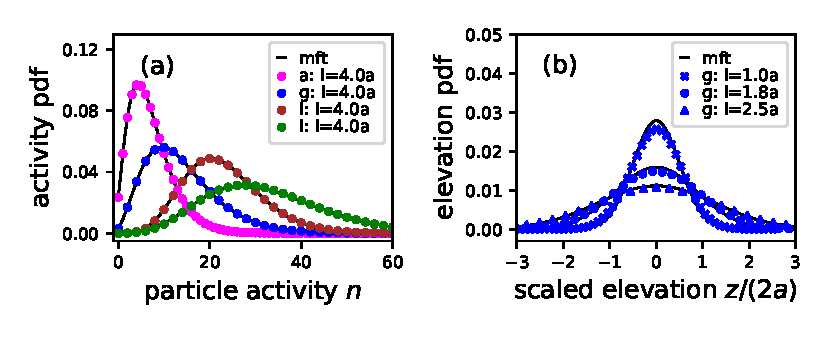
\includegraphics[width=\linewidth,keepaspectratio]{distributions.pdf}
	\caption{Panel (a) presents the probability distribution of particle activity $n$ and panel (b) presents the probability distribution of the relative number of particles $m$ for a representative subset of simulations. These distributions represent different flows from table \ref{tab:anceyparams}, distinguished by color, and different values of the active layer depth $l$ (equivalently the coupling constant $\kappa$), distinguished by the marker style. The mean field theories (mft) of equations (\ref{eq:ancey}) and (\ref{eq:ou2}) are displayed as solid black lines.}
	\label{fig:pdfs}
\end{figure}
The mean field equation (\ref{eq:ancey}) for the particle activity $n$ closely represents the numerical results, and while there are small differences between numerical and analytical results for the relative number $m$ of resting particles, the numerical solutions approximately match equation (\ref{eq:ou2}), having Gaussian profiles consistent with our assumption of a symmetric scaling of erosion and deposition rates with bed elevation changes. 


\subsection{Statistical moments}
\label{sec:mom}

We calculate the moments of $n$ and $m$ by summing over $P(n,m)$. 
The $j$th order unconditional moment of the particle activity $n$ derives from
\begin{equation} \langle n^j \rangle = \sum_{n}n^jP(n),\end{equation}
while the $j$th order moment of $n$ held conditional on $m$ is
\begin{equation} \langle n^j|m \rangle = \sum_{n}n^j P(n,m) .\end{equation}
\begin{wrapfigure}{r}{0.5\textwidth}
	\centering
	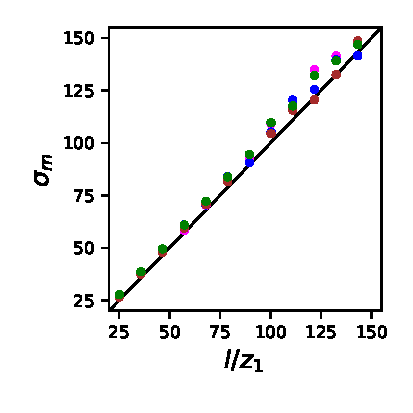
\includegraphics[width=0.5\textwidth,keepaspectratio]{variance.pdf}
	\caption{Data from all simulations demonstrating that the active layer depth $l$ characterizes bed elevation changes as posited in equation (\ref{eq:active}): $\sigma_m^2 \approx (l/z_1)^2$. }
	\label{fig:var}
\end{wrapfigure}
We observe no dependence of the moments of $m$ on the value of $n$. 
The mean elevation is always $\langle m \rangle = 0 $ due to our initial assumption of symmetry in the entrainment and deposition rate scaling with $m$. 
Figure \ref{fig:var} demonstrates that the variance of bed elevations is approximately $\sigma_z^2 = z_1^2 \sigma_m^2 = \frac{1}{4\kappa}=l^2$, agreeing with the approximation in equation (\ref{eq:ou2}); this result supports our earlier assertion that $l$ is a characteristic length scale of bed elevation fluctuations.
The close correspondence between the mean field approximation and the numerical simulations in figure (\ref{fig:pdfs}a) suggests the unconditional moments of $n$ correspond closely with the \citet{Ancey2008} result. We find them to be identical within numerical uncertainty.

The coupling between bed elevation changes and the erosion and deposition rates develop a strong dependence of the particle activity on $m$. Figure (\ref{fig:condmoms}) displays the mean shift $[\langle n |m \rangle - \langle n \rangle]/\langle n \rangle $ and the variance shift  $[\text{var}(n|m) - \text{var}(n)]/\text{var}(n)$ of the particle activity due to departures of the bed elevation from its mean position.
\begin{figure}[!ht]
	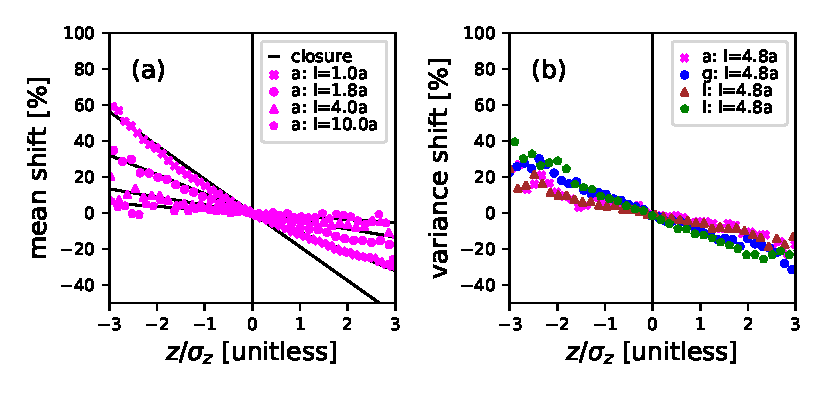
\includegraphics[width=\linewidth,keepaspectratio]{momentsuppression.pdf}
	\caption{The shifts between particle activity moments conditioned on instantaneous elevations and their over-all mean values. Panel (a) indicates the mean particle activity shift versus the bed elevation measured in units of $\sigma_z=l$. This shift displays asymmetric dependence on $m$ at the flow conditions of the \citet{Ancey2008} experiements, and departures of the bedload transport mean can be as much as 60\% when the bed is in a severely degraded state with $z\approx -3l$. The closure equation (\ref{eq:closure}) is plotted in panel (a) Panel (b) demonstrates a more symmetrical variance shift with some dependence on flow conditions displaying shifts of up to 20\% with bed elevations. These results indicate that bedload statistics measurements on short timesclaes could be severely biased by departures from the mean bed elevation.}
	\label{fig:condmoms}
\end{figure}
Figure (\ref{fig:condmoms}a) demonstrates that the \citet{Ancey2008} flow conditions support departures of the mean particle activity by as much as 60\% from the overall mean value when the bed is in a degraded state $z\approx -3l$, and the activity can be decreased by 20\% when the bed is in an aggraded state.
The closure model (\ref{eq:closure}) used to derive the approximate bed elevation distribution (\ref{eq:ou2}) is plotted behind the conditional mean profiles in figure (\ref{fig:condmoms}a), where it appears to be crude approximation, as it does not capture the asymmetry in this quantity.
Nevertheless, figure \ref{fig:var} demonstrates the variance $1/(4\kappa)$ derived from this closure equation is representative of the numerical relationship.
For the parameters of the \citet{Ancey2008} experiments, figure (\ref{fig:condmoms}b) displays a variance shift with bed elevation changes that is less severe than the mean shift but is nevertheless appreciable, with bed elevations changing the magnitude of bedload activity fluctuations by as much as 20\%.
We summarize that bed elevation changes regulate the particle activity moments, with a moment suppression effect when the bed is aggraded, and a moment enhancement effect when the bed is degraded.

\subsection{Collective entrainment and bedload activity fluctuations}
\label{sec:colent}
Noting that bed elevations regulate the particle activity moments, we now study the influence of collective entrainment on this effect by modifying the relative proportion of the individual to collective contributions in the mean entrainment rate $E=\lambda + \sigma \langle n \rangle $.
Using the equilibrium condition $E=D$, we determine the fraction of entrainment due to the collective process is $f = \mu\langle n \rangle/E = \mu/\sigma$. Using this fraction, we can hold $E$ constant and modify the prevalence of the collective entrainment process by setting $\lambda = E(1-f)$ and $\mu= \sigma f$. As we interpolate $f$ between zero and one, the particle activity component of the master equation \ref{eq:master} interpolates from a purely Poissonian model \citep{Ancey2006} to a negative binomial model \citep{Ancey2008}, isolating the imprint of collective entrainment on particle activity statistics over a dynamic sedimentary bed.
\begin{figure}[!ht]
	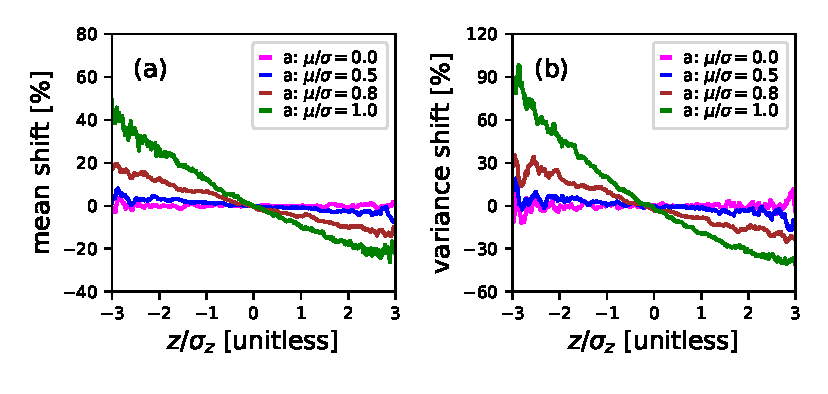
\includegraphics[width=\linewidth,keepaspectratio]{colent-suppression.pdf}
	\caption{The shift of the mean particle activity in panel (a) and its fluctuations in panel (b) with departures of the bed elevation from its mean. All simulations are at flow condition (g) from table \ref{tab:anceyparams} except $\lambda$ and $\mu$ are modified to shift the fraction $f=\mu/\sigma$ of the over-all entrainment rate $E$ due to collective entrainment. Clearly, collective entrainment drives strong departures of the bedload statistics away from the mean field model (\ref{eq:ancey}) at large departures from the mean bed elevation. Panel (b) shows particle activity fluctuations suppressed by 90\% when $z\approx -3l$ and collective entrainment is the dominant process. When collective entrainment is absent, meaning $\mu/\sigma=0$, this moment regulation effect vanishes: it is a consequence of collective entrainment.}
	\label{fig:colent}
\end{figure}
Figure \ref{fig:colent} depicts the modification of the particle activity mean and variance as the importance of collective entrainment is tuned (through $\lambda$ and $\mu$) with all other parameters fixed. When $f=0$, the bed elevation ceases to influence the particle activity mean or variance, while larger fractions increasingly enable the moment regulation effect we introduced in section \ref{sec:mom}.

\subsection{Resting times of sediment undergoing burial}
\label{sec:rtcdf}

\begin{figure}[!ht]
	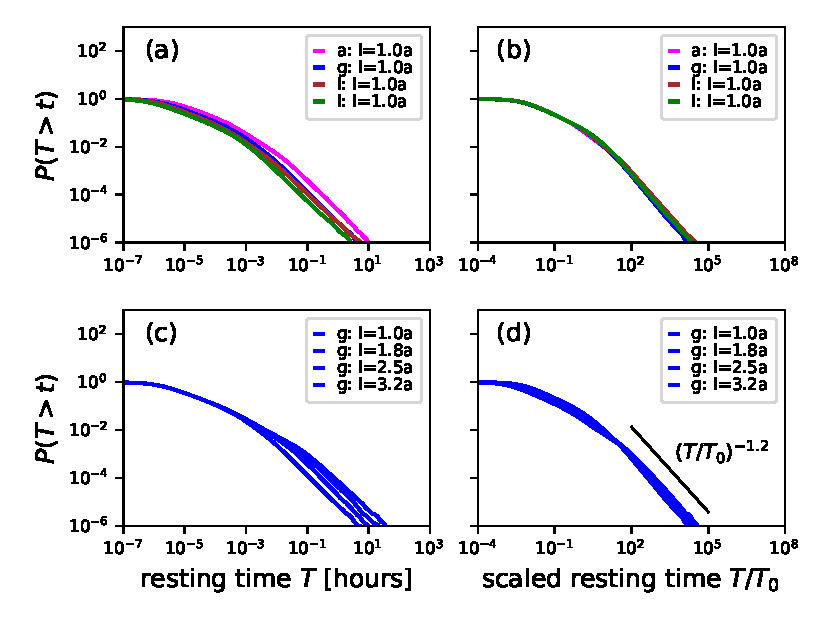
\includegraphics[width=\linewidth,keepaspectratio]{rtcdf.pdf}
	\caption{Resting time statistics scale differently with transport conditions and the bed elevation variance. Panel (a) shows differing flow conditions at a fixed $l$ value, while panel (c) shows fixed flow conditions at differing $l$. When scaled by $T_0$ (\ref{eq:time}), both types of difference collapse in the tails of the distributions, as shown in panels (b) and (d). In panels (b) and (d), the black dotted lines indicate a power law decay of the collapsed tails having parameter $\alpha\approx1.18$ .}
	\label{fig:cdfs}
\end{figure}

Resting times for sediment undergoing burial are obtained from analyzing the return times from above in the time-series of $m$ \citep[e.g.,][]{Redner2007}.
Following \citet{Voepel2013} and \citet{Martin2014}, we concentrate on a particular bed elevation $m'$, and find all time intervals separating deposition events at $m=m'$ from erosion events at $m=m'+1$.
These are the return times from above of the sedimentary bed conditional to the elevation $m'$.
Binning these conditional return times (using logarithmically-spaced bins to reduce computational load) and counting the occurrences in each bin, we obtain an exceedance distribution of return times $t_r$ held conditional to the elevation $m'$: $P(T>t_r|m')$.
Using the marginal probability distribution of bed elevations $P(m)$ (figure \ref{fig:pdfs}(b)), we derive the unconditional exceedance distribution of resting times as a sum over all elevations \citep{Yang1971, Nakagawa1980, Voepel2013, Martin2014}: 
\begin{equation} P(T>t_r) = \sum_{m'} P(m') P(T>t_r|m') .\end{equation}
A representative subset of these results are displayed in figure \ref{fig:cdfs}.
Comparing panels \ref{fig:cdfs}(a) and \ref{fig:cdfs}(c) shows two separate variations with input parameters: first, the distributions vary with the flow conditions, and second, they vary with the standard deviation of bed elevations ($l$).
However, as shown in panels \ref{fig:cdfs}(b) and \ref{fig:cdfs}(d), a characteristic timescale $T_0$ is found to collapse away both variations.
We obtained this $T_0$ heuristically by considering the characteristic speed of bed elevation change.
This is the mean number of grains leaving the bed per unit time is $E$, and the removal of a single grain changes the bed elevation by $z_1$ (\ref{eq:ele}). 
Therefore, bed elevations change with a characteristic speed $v = z_1 E$.
Since the range of elevation deviations is $l$ (figure \ref{fig:var}), the time required for the bed to shift through this characteristic distance is $l/v$, or equivalently
\begin{equation} T_0 = \frac{l}{z_1 E}.\label{eq:time}\end{equation}
When scaling the resting time by this $T_0$, we obtain the collapse shown in figure \ref{fig:cdfs}.
Using the log-likelihood estimation technique described by \citet{Newman2005}, we estimate the scaled resting time non-exceedance distributions decay as a heavy tailed power law with parameter $\alpha = 1.18 \pm 0.32$ for all return times satisfying $T/T_0 > 10^3$.
These distributions are sufficiently heavy tailed to violate the central limit theorem and drive anomalous super-diffusion of bedload, a result which supports the earlier conclusions of \citet{Voepel2013} and \citet{Martin2014}.

\section{Discussion}
\label{sec:discussion}

\subsection{Context}
Einstein developed the first stochastic models of bedload tracer diffusion \citep{Einstein1937} and the bedload flux \citep{Einstein1950}, and his ideas can be viewed as the nexus of an entire paradigm of research that extends into the present day \citep[e.g.,][]{Hubbell1964, Nakagawa1976,Hassan1991,Ancey2008, Wu2019}.
These models aim to predict bedload transport characteristics from stochastic concepts of individual particle motions.
With some exceptions \citep{Yang1971,Nakagawa1980,Pelosi2016,Wu2019,Wu2019a}, existing descriptions are spatially one-dimensional, concentrating on the motion of grains in the downstream direction without including the vertical dimension wherein local bed elevation changes imply sediment burial \citep{Voepel2013,Martin2014} and change the mobility of surface grains \citep{Yang1971,Nakagawa1980}.

\subsection{Contributions}

In this paper, we have built on earlier works \citep{Ancey2008,Martin2014} to include the vertical dimension of bed elevation dynamics, study the interplay between bedload transport and bed elevation fluctuations, and investigate resting time distributions of sediment undergoing burial.
To our knowledge, this model is the first description of bedload transport and bed elevations as a coupled stochastic population model based on individual grains.
Numerical solutions and analytical approximations provided negative binomial distributions of bedload activity and normal distributions of bed elevations.
Although experiments under more natural conditions with segregation processes,  migrating bedforms, or sediment supply perturbations have shown particle activity distributions with heavier tails \citep{Dhont2018,Saletti2015a} and non-Gaussian bed elevations \citep{Singh2012,Aberle2006}, our results reproduce the key features of the most controlled bed elevation \citep{Wong2007,Martin2014} and bedload transport \citep{Heyman2016,Ancey2008} experiments in the literature.

Our inclusion of coupling between the bed elevation and entrainment and deposition rates revealed a novel dependence of particle activity on bed elevation changes,  highlighting a new consequence of the collective entrainment process \citep{Ancey2008,Lee2018}. This coupling develops a significant variation of the particle activity moments with deviations of the bed from its mean elevation. We isolated the role of collective entrainment in this bedload activity regulation, and pointed out that particle activity variations with bed elevations dissapear in the absence of collective entrainment.
Finally, we obtained resting times for sediment undergoing burial within the sedimentary bed by analyzing return times from above in the bed elevation time-series. We found heavy-tailed power law resting times with tail parameters sufficient to drive anomalous diffusion of bedload at long timescales.
The distribution tails were found to collapse across flow conditions using a timescale formed from the mean erosion rate and the active layer depth.

As our model builds on earlier works describing particle activity and bed elevation changes independently, it also reduces to these works in simplified limits when the coupling between the particle activity and bed elevation vanishes.
With the mean field approach in section \ref{sec:analytical}, we derived the \citet{Martin2014} Ornstein-Uhlenbeck model for bed elevations and the \citet{Ancey2008} birth-death model for the particle activity as simplified limits of our coupled model. While the mean field description of bed elevations over-predicts the bed elevation variance by approximately a factor of two, it does capture the Gaussian shape of the bed elevation distribution, and its conclusions on the tail characteristics of resting time distributions for sediment undergoing burial are identical to ours within the numerical uncertainty: \citet{Martin2014} described a power-law distribution with tail parameter $\alpha \approx 1$ which falls neatly within our estimation $\alpha = 1.18 \pm 0.32$. In addition to our original contributions, we have corroborated the models of \citet{Ancey2008} and \citet{Martin2014} from an alternate perspective, showing their results to be mostly robust when accounting for bed elevation changes.


\subsection{Next steps}

The model we have presented computes statistical characteristics of the bedload particle activity and bed elevation within a control volume by assuming all particles on the bed surface have similar mobility characteristics while sediment transport and bed topography are in equilibrium. In actuality, particles span a range of sizes, and spatial organization occurs both in the forces imparted to particles by the flow \citep{Shih2017,Amir2014} and in the mobility characteristics of particles on the bed surface \citep{Charru2004, Hassan2008, Nelson2014}.
Together, these factors may generate spatial correlations in particle activities that models concentrating on a single control volume will be unable to capture. 
Models chaining multiple control volumes together have shown spatial correlations in the particle activity as a result of collective entrainment \citep{Heyman2014, Ancey2015}, and similar approaches have also been applied to study correlations in turbulent flows \citep{Gardiner1983}. In light of this work, we consider the model we have presented as a preliminary step toward a multiple-cell model of particle activities and bed elevation changes with potential to express spatial correlations between longitudinal profile and particle activity statistics.

Like \citet{Martin2014}, we obtained heavy-tailed power-law resting times for sediment undergoing burial by treating bed elevation changes as an unbounded random walk with a mean reverting tendency.
This result suggests sediment burial can explain the heavy-tailed rests seen in field data \citep{Olinde2015,Bradley2017,Pretzlav2016}. 
Our resting time distributions show a divergent variance and possibily a divergent mean, since this occurs for $\alpha < 1$ \citep{Sornette2000} which is within range of our results.
Divergent mean resting time distributions present a paradox, since they imply all particles should eventually be immobile, violating the equilibrium transport assumption.
\citet{Voepel2013} demonstrated that a bounded random walk for bed elevations provides a power-law distribution that eventually transitions to a faster thin-tailed decay, allowing for power-law scaling like our result and \citet{Martin2014} without this divergent mean paradox. 
One resolution to this issue could come from a spatially distributed model with multiple cells. Neighboring locations might bound excessive local elevation changes through granular relaxations from gradients above the angle of repose. In this interpretation, divergent mean power law resting time distributions may be relics of single cell models for bed elevation changes. We should always expect a maximum depth to which the bed can degrade relative to neighboring locations; this could temper the power law tail without required the reflecting boundaries used by \citet{Voepel2013}.

Finally, we studied probability distribution functions and first and second moments of the particle activity and bed elevation, making novel conclusions about coordination between the statistical characteristics of these quantites which deserve experimental testing.
In the last decade, particle tracking experiments have emerged \citep{Lajeunesse2010,Roseberry2012,Martin2014, Fathel2015,Heyman2016,Liu2019}, that allow joint resolution of bed elevations and bedload transport. 
A suitably designed experiment could test our prediction that bed elevations regulate particle activity statistics, as essentially represented in figures \ref{fig:condmoms} and \ref{fig:colent}. 
However, we have left many other statistical characteristics of bedload transport for future studies. 
For example, the dependence of bedload transport \citep{Saletti2015a,Singh2009} and bed elevation statistics \citep{Aberle2006, Singh2009,Singh2012} on the spatial and temporal scales over which they are observed is an emerging research topic. Statistical quantities can either be monoscaling or multiscaling across the observation scale \citep{Sornette2000}, and we currently lack physical understanding and general conclusions about the scale dependence of particle activity and bed elevation signals.
The model we have presented shows statistical monoscaling for both quantites \citep[e.g.][]{Saletti2015a}, whereas other experiments indicate statistical multiscaling \citep{Aberle2006,Singh2009,Singh2012}. We consider this topic to go beyond the scope of the present work, and we have focused on statistical characteristics at the highest temporal resolutions, with no averaging over the observation scale.

\section{Conclusion}
\label{sec:conclusion}

We developed a stochastic model for particle activity and local bed elevations including feedbacks between elevation changes and the erosion and deposition rates.
This model includes collective entrainment, whereby moving particles tend to destabilize stationary ones.
We analyzed this model using a mixture of numerical and analytical methods and provided two key results:
\begin{enumerate}
\item Resting times for sediment undergoing burial lie on a heavy-tailed power law distributions with tail parameter $\alpha \approx 1.2$;
\item Collective entrainment generates a statistical regulation effect, whereby bed elevation changes modify the mean and variance of the particle activity by as much as 90\%: this effect vanishes when collective entrainment is absent.
\end{enumerate}
These results imply measurements of bedload transport statistics could be severely biased at observation timescales smaller than adjustments of the bed elevation timeseries when collective entrainment occurs.
Next steps are to generalize our model to a multi-cell framework and to study spatial correlations in bed elevation and particle activity statistics.


\acknowledgments
The simulation code is available at
\sloppy
\url{https://drive.google.com/file/d/1bWEX_ZHlcGRKCxtRIadnSbhh4EpQlsoh/view?usp=sharing}.
This research was supported by an NSERC Discovery Grant to M. Hassan.
We would like to thank Shawn Chartrand and Conor McDowell for helpful discussions.

\bibliography{biblio}
\end{document}

